\documentclass{ximera}
%% handout
%% nohints
%% space
%% newpage
%% numbers

%% You can put user macros here
%% However, you cannot make new environments

\graphicspath{{./}{firstExample/}{secondExample/}}

\usepackage{url}
\usepackage{tikz}
\usepackage{tkz-euclide}
\usetkzobj{all}


\tikzstyle geometryDiagrams=[ultra thick,color=blue!50!black]
\pgfplotsset{compat=1.8}
  \usepackage[T1]{fontenc}
  \usepackage[utf8x]{inputenc}



\title{Expected value}

\begin{document}
\begin{abstract}
We introduce the idea of the expected value of a situation and compute some examples.
\end{abstract}
\maketitle

\subsection*{Basic learning objectives}

These are the tasks you should be able to perform with reasonable fluency \textbf{when you arrive at our next class meeting}. Important new vocabulary words are indicated \emph{in italics}. 

\begin{itemize}
	\item Understand the definition of the \emph{expected value} of a situation.
    \item Understand the interpretation of the expected value.
    \item Compute the expected value of a simple probabilistic game.
\end{itemize}

\subsection*{Advanced learning objectives}

In addition to mastering the basic objectives, here are the tasks you should be able to perform \textbf{after class, with practice}: 

\begin{itemize}
    \item Compute the expected value of more complex probabilistic games.
    \item Compute the \emph{house edge} of simple gambling games.
\end{itemize}

Imagine you have a fair coin and that you're going to play the following gambling game with a ``friend'' that we will name ``the casino.'' The rules are simple:
\begin{itemize}
  \item If the coin comes up heads, the casino pays you \$1.
  \item If the coin comes up tails, you pay the casino \$1.
\end{itemize}
Setting aside any moral qualms you might have against gambling, you should be able to recognize that this game is fair. But what makes it fair? Most people respond with the idea that you have an equal chance of winning and losing.

But let's change the game a bit. What if you were playing with the following rules:
\begin{itemize}
  \item If the coin comes up heads, the casino pays you \$0.99.
  \item If the coin comes up tails, you pay the casino \$1.
\end{itemize}
Something about this should feel unfair. The unfairness doesn't have anything to do with the frequency with which you win and lose, but how much you win or lose when you win or lose.

Up to think point, we've really only been talking about probabilities. But when you include some form of score-keeping like money, the problem becomes more complicated. This added feature leads us to the concept of \emph{expected value}. The expected value of a game is how much you expect to win or lose on average when playing the game once.

For example, if the expected value of a game is \$$1$, then you expect to win \$$1$ \emph{on average}. This doesn't mean that you will win \$$1$ every single time, and it may turn out that it's impossible for you to win exactly \$$1$. But if you play the game many times and average the results, you expect to average a \$$1$ win for each game.

The formula for expected value looks complicated, but it's not that bad:
\[ E[X] = \sum P(X_i) \cdot V(X_i). \]
What does this mean?
\begin{itemize}
  \item The symbol $\sum$ is called a summation symbol and it indicates that you are to add up several terms, described by the symbols to the right of the summation sign.
  \item The symbol $E[X]$ is the expected value of the game $X$.
  \item The $X_i$ is a notation that represents all the possible outcomes of the game $X$.
  \item The $P(X_i)$ is the probability of the event $X_i$, just as before.
  \item The $V(X_i)$ is the \emph{value} of the event $X_i$. This is the amount of points or money the player wins when event $X_i$ happens.
\end{itemize}

That's a lot of notation to take in, but after working through an example, it will make more sense. We will compute the expected value of the second game above (where you only win \$0.99 when you win).

For this game, $i$ takes on only $2$ values beause we have the following events:
\[ \begin{array}{cc}
      X_1 = \text{``H''} & X_2 = \text{``T''} 
\end{array} \]
Since we know the coin is fair, we know the probability of each event is the same:
\[ \begin{array}{cc}
      P(X_1) = \frac{1}{2} & P(X_2) = \frac{1}{2}
\end{array} \]
And we can read off the value of each event from the description of the game. Notice that when the casino wins, we have a negative value because we're measuring this game relative to the player. We also drop the dollar sign because it clutters the notation.
\[ \begin{array}{cc}
      V(X_1) = 0.99 & V(X_2) = -1
\end{array} \]

This information can be put into a probability tree. The values are listed at the end of the branches.

\begin{image}
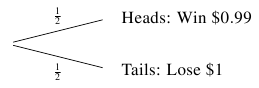
\includegraphics{ExpectedValue1.png}
%\tikzstyle{level 1}=[level distance=2cm, sibling distance=1cm]
%\tikzstyle{level 2}=[level distance=2cm, sibling distance=.75cm]
%\begin{tikzpicture}[grow=right]
%\node{}
%    child {
%       	node[label=right:{Tails: Lose \$$1$}] {}
%        edge from parent
%        node[below] {\footnotesize $\frac{1}{2}$}
%    }
%    child {
%       	node[label=right:{Heads: Win \$$0.99$}] {}
%        edge from parent
%        node[above] {\footnotesize $\frac{1}{2}$}
%    };
%  \end{tikzpicture}
\end{image}

We can now compute the expected value:
\begin{align*}
  E[X] & = \sum P(X_i) \cdot V(X_i) \\
    & = P(X_1) \cdot V(X_1) + P(X_2) \cdot V(X_2) \\
    & = \frac{1}{2} \cdot (0.99) + \frac{1}{2} \cdot (-1) \\
    & = -0.005
\end{align*}

What does this mean? It means that on average, each time you play this game you will lose half of a cent. This may not seem like much, but if you play this game over and over again, the casino will eventually have all of your money.

\begin{question}
What is the expected value of a game?

    \begin{multipleChoice}
      \choice{How often you expect to win the game.}
      \choice[correct]{How much you expect to win or lose on average when playing the game once.}
      \choice{How much you win when you win the game.}
    \end{multipleChoice}

\end{question}

\begin{question}
The symbol $\sum$ represents which arithmetic operation?

    \begin{multipleChoice}
      \choice[correct]{Addition}
      \choice{Subtraction}
      \choice{Multiplication}
      \choice{Division}
    \end{multipleChoice}

\end{question}

\begin{question}
Determine the expected value of the following game: You flip a fair coin. If it comes up heads, you win \$$100$. If it comes up tails, you lose \$$80$.

    \begin{multipleChoice}
      \choice{$\$100$}
      \choice{$-\$80$}
      \choice{$\$20$}
      \choice[correct]{$\$10$}
      \choice{$-\$20$}
    \end{multipleChoice}
    \begin{hint}
      Draw the probability tree and label it like the example.
    \end{hint}
    \begin{hint}
      Match up the symbols in the expected value formula with the parts of the problem to make sure everything matches.
    \end{hint}

\end{question}

\end{document}
